\section{半导体的晶体结构}

\subsection{金刚石结构}
重要的半导体材料,包括硅\xce{Si}、锗\xce{Ge}等在化学元素周期表中都属于第\Romnum{4}族元素,原子的最外层都具有$4$个价电子。硅原子和锗原子组成晶体时依靠的是共价键的结合,它们的晶格结构与碳原子构成的金刚石结构一致,关于金刚石结构,我们在固体物理中已经有了比较清楚的认识,简而言之,每个原子的四个最近邻原子以正四面体的方式分布,即配位数为$4$。

金刚石结构可用\xref{fig:金刚石结构的俯视投影}的俯视投影表示,对比固体物理中的立体图很容易理解
\begin{Figure}[金刚石结构的俯视投影]
    \includegraphics[scale=0.55]{build/Chapter01A_01.fig.pdf}
\end{Figure}
\xref{fig:金刚石结构的俯视投影}中,虚线是晶胞边界,数字是该原子距晶胞顶面的距离(几倍晶格常数)。

金刚石结构的共价键晶体中,每个原子的$4$个共价键是完全等价的,这是怎么实现的呢?实际上,它们是由$1$个s态和$3$个p态线性组合而成的$4$个sp$^{3}$杂化轨道,键角为$109^\circ 28'$。

金刚石的每个晶胞中,共有$8$个原子(顶点$1$个、侧面$3$个、内部$4$个),实验测得
\begin{Table}[硅和锗的晶体参数]{lrrrr}
    <元素&晶格常数(\si{nm})&单位体积原子(\si{cm^3})&原子最短间距(\si{nm})&原子的共价半径(\si{nm})\\>
    硅&$0.543102$&$5.00\times 10^{22}$&$0.235$&$0.117$
    \\
    锗&$0.565791$&$4.42\times 10^{22}$&$0.245$&$0.122$\\
\end{Table}
由晶格常数$a$可知晶格体积为$a^3$,单位体积的晶格数即$1/a^3$,单位体积的原子数即$8/a^3$,考虑导金刚石的每个晶胞具有$8$个原子(特别注意单位换算,上述单位体积是单位立方厘米)。

\subsection{闪锌矿和纤锌矿结构}
实际上,除了硅和锗这样的半导体,许多\Romnum{3}--\Romnum{5}族化合物和\Romnum{2}--\Romnum{6}族化合物都是半导体。

化合物半导体通常有两种主要构型
\begin{itemize}
    \item 闪锌矿结构,主要出现在化合键中共价键成分比较高的情况。
    \item 纤锌矿结构,主要出现在化合键中离子键成分比较高的情况。
\end{itemize}
化合物中,\Romnum{3}--\Romnum{5}族呈闪锌矿结构,\Romnum{2}--\Romnum{6}族则能以闪锌矿和纤锌矿两种方式结晶。

\begin{Figure}[纤锌矿结构]
    \vspace{-0.5cm}
    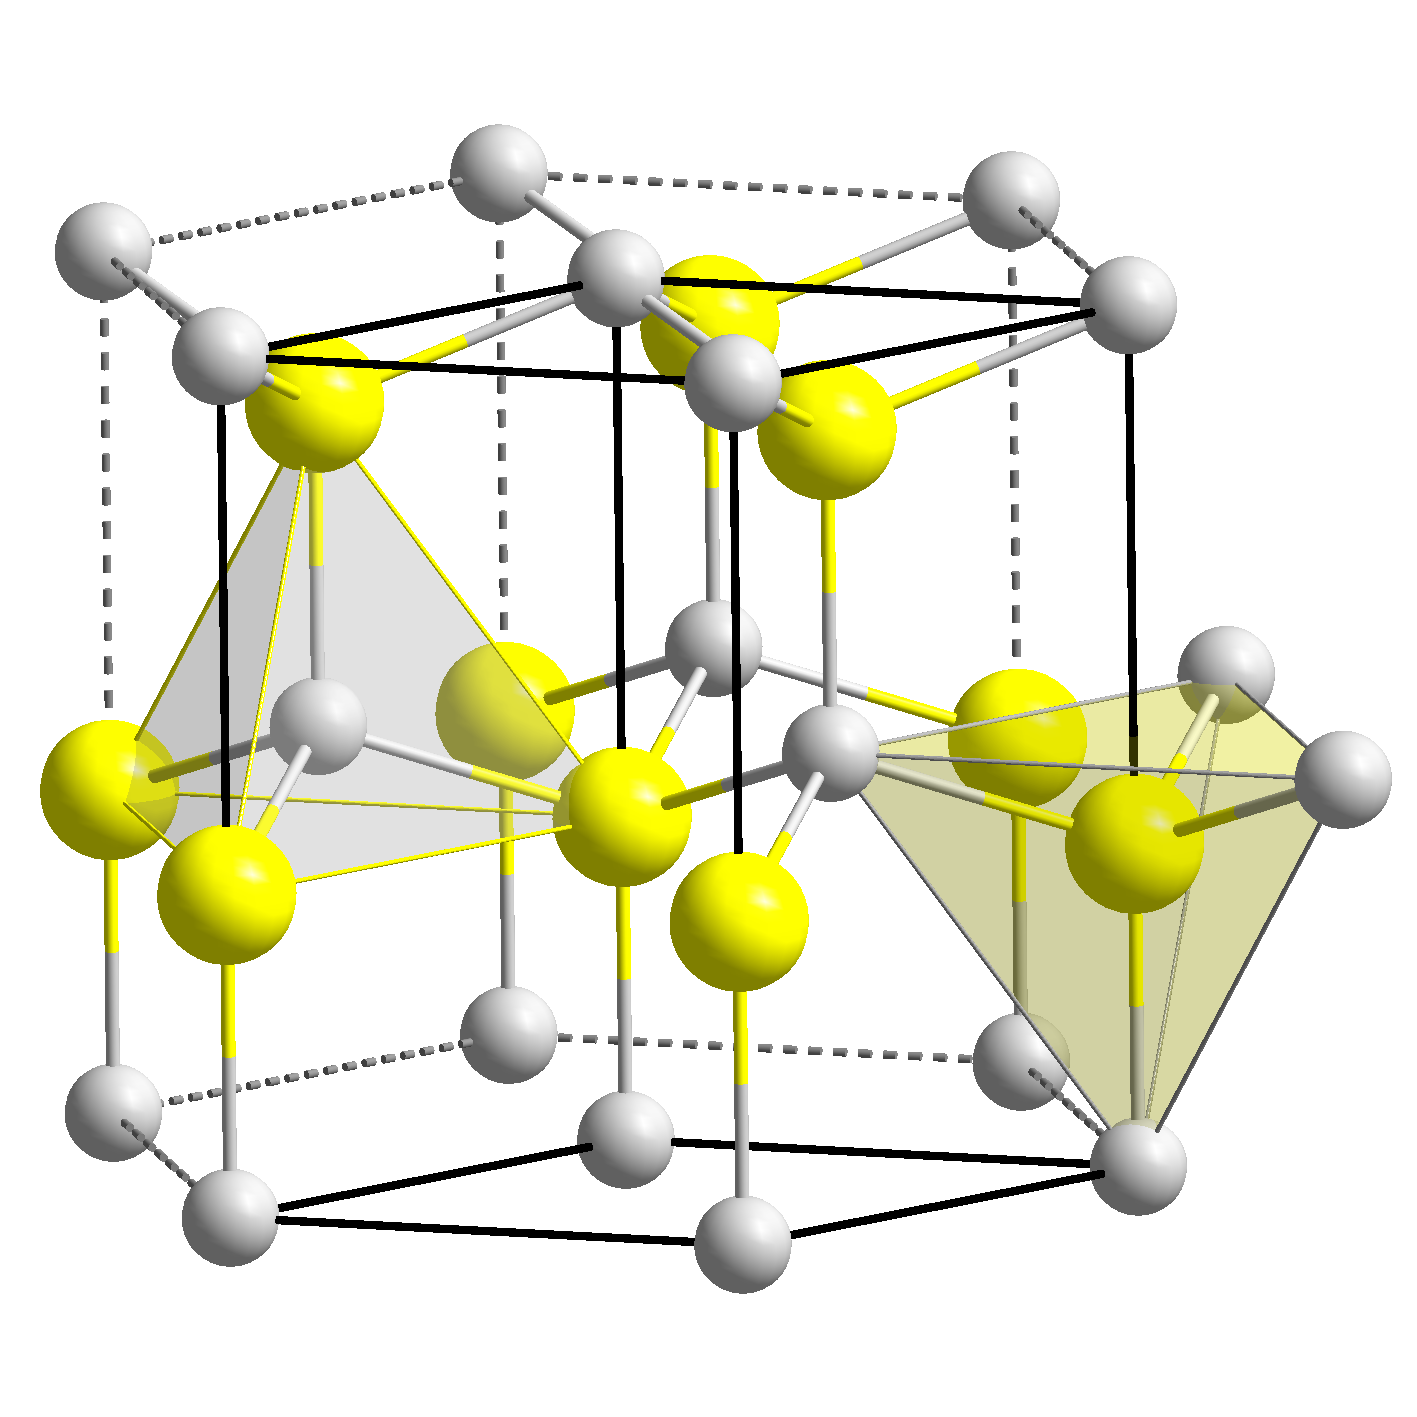
\includegraphics[width=6cm]{image/Wurtzite_polyhedra.png}
    \vspace{-0.5cm}
\end{Figure}

闪锌矿结构是我们在固体物理中比较熟悉的,它与金刚石结构非常相似,但不同的是,闪锌矿结构中$A,B$两类原子分别由化合物中的两种不同原子构成。纤锌矿结构则是一种新的晶体结构,如\xref{fig:纤锌矿结构}所示\cite{W1},纤锌矿结构和闪锌矿结构一样,两类原子都位于对方构成的正四面体的中心,但是,纤锌矿具有六方对称性,具体的说,两类原子自身先构成六角点阵(这里六角点阵上下底面的中间还有三个格点),随后,两类原子的点阵上下将错开略小于$c/2$的距离,这里$c$是六角点阵的高,而准确的错开距离,即略小于$c/2$多少由构成正四面体的要求确定。